\chapter{Evaluierung Permissioned Blockchains für B2B}
\label{cha:b2b-eval}

Die Blockchain-Technologie bringt diverse Probleme mit sich, welche je nach Anwendungszweck und Blockchaintyp verschieden große Auswirkungen haben. Für den B2B-Bereich gilt es vor allem die Skalierbarkeit sowie die Konsensmechanismen zu analysieren.


\section{Skalierbarkeit}
\label{sec:scalability-eval}
Das CAP-Theorem besagt, dass es in einem verteilten System nur möglich ist, 2 von den 3 folgenden Eigenschaften zu erfüllen: Konsistenz, Verfügbarkeit und Ausfalltoleranz. Bei der Blockchain wären dies: Dezentralisierung, Skalierbarkeit und Nichtangreifbarkeit \cite{SchererPerformanceScalabilityBlockchain2017}. Im Bezug auf die Skalierbarkeit wird vor allem auf den Transaktionsdurchsatz sowie die Bestätigungszeiten von Transaktionen eingegangen. Dazu erfolgt zunächst eine Analyse an aktuellen Public Blockchains, und letztendlich an Permissioned Blockchains. Die Ergebnisse werden ebenfalls auf das CAP-Theorem angewandt.  

\subsection{Public Blockchains}

\begin{figure}[htb]
  \centering
    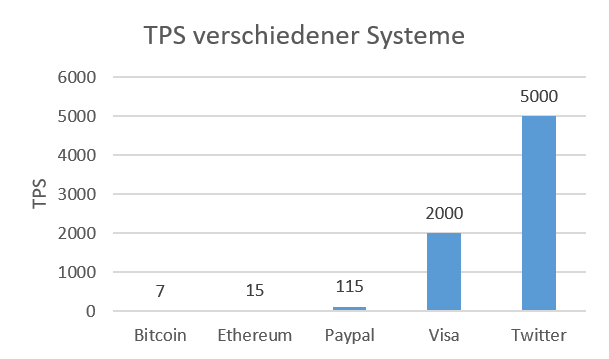
\includegraphics[width=0.95\textwidth,angle=0]{images/tps-comparison}
     \caption{Möglicher Transaktionsdurchsatz bei Bitcoin, Ethereum, Paypal und Visa \cite{ScalabilityBitcoinWiki}.}
    \label{fig:tps-comparison}
\end{figure}

%TODO: Bitcoin-Kapitel nochmal unterteilem in paragraphs ?
\subsubsection{Bitcoin}
%TODO: Transaktionsgebühren erwähnen ?
Das Bitcoin-Netzwerk erreicht aktuell einen maximalen Transaktionsdurchsatz von 7 Transaktionen (Unterschiedlich je nach Größe der Transaktionen) pro Sekunde (TPS), bei einer Blockgröße von 1MB.  Hingegen erreicht Paypal 115 TPS, und Visa 2000 TPS (Siehe auch Abb. \ref{fig:tps-comparison}) \cite{ScalabilityBitcoinWiki}. Hinzu kommt, dass ungefähr 170000 unbestätigte Transaktionen\footnote{Unbestätigte Transaktion: Eine Transaktion, welche noch nicht in einen Block vorkommt \cite{AntonopoulosMasteringbitcoin2015}} bestehen \cite{BlockchainFirmaBlockchainChartsUnbestatigte}. Berechnungen von Scherer zeigen, dass bei 11,8 Millionen Nutzern im Bitcoin-Netzwerk, sowie einem Transaktionsdurchsatz von 4 TPS, jeder Nutzer nur nur ca. 10 Transaktionen im Jahr senden kann \cite{SchererPerformanceScalabilityBlockchain2017}.

%TODO: SegWit ?
Der Transaktionsdurchsatz ist durch verschiedene Faktoren limitiert. Hauptsächlich durch die limitierte Blockgröße von 1MB, und dem Proof-of-Work: Nur eine bestimmte Anzahl an Transaktionen passt in einen Block, und nur alle 10 Minuten wird einer erstellt. Es gäbe also die Möglichkeit, die Blockgröße zu vergrößern, oder die Zeit für den Proof-of-Work zu verringern, indem die Schwierigkeit angepasst wird. Es gibt jedoch diverse Nachteile, welche dadurch entstehen würden. Bei einer größeren Blockgröße würde es länger dauern, bis ein Block beim Propagieren durch das Netzwerk alle Nodes erreicht. Dies würde zu öfter vorkommenden und längeren Forks führen und somit die Sicherheit des Netzwerks beeinträchtigen. Den gleichen Effekt hätte eine kürzere Proof-of-Work Zeit, da die Wahrscheinlichkeit höher ist, dass zwei Nodes zur ungefähr gleichen Zeit einen Block erstellen \cite{SchererPerformanceScalabilityBlockchain2017} \cite{EthereumWhitepaper2017} \cite{SompolinskyAcceleratingBitcoinTransaction2013}. 

%TODO: Erhöhte Chance auf Angriff/Double Spend erwähnen ?
Entsteht ein Fork, probieren Nodes die längere und somit gültige Blockchain zu erschaffen. Gelingt dies, wird die kürzere Blockchain mit den nun sogenannten Stale Blocks verworfen. Die gesamte Rechenleistung, welche in die Stale Blocks und seine Nachfolger geflossen ist, trägt nicht zur Sicherheit des Netzwerks bei. Dies lässt sich auch anhand der Abbildung \ref{fig:forking-risks} erläutern. Innerhalb der Blockchain bestehen durch mehrere Forks 5 Branches. Das bedeutet, dass die Rechenleistung des Netzwerks auf diese aufgespalten ist. Es wird davon ausgegangen, dass 20\% der Rechenleistung in den obersten Branch geflossen ist, welcher der längste ist. Die restlichen 4 Branches erhalten je 10\% der Rechenleistung. Wenn es nun einen Angreifer mit 40\% der Rechenleistung probiert eine eigene Blockchain zu erstellen, gelingt ihm dies, da er schneller die längere Blockchain erstellen kann \cite{SompolinskyAcceleratingBitcoinTransaction2013}. Zusammenfassend lässt sich sagen, dass ein Angreifer nicht 51\% der Rechenleistung für einen Fork benötigt, wenn das Netzwerk diese bei Forks verschwendet \cite{Buterin12secondBlockTime2014}. 

Ein weiteres Problem der Forks ist, dass Miner keine Belohnung für die Arbeit an verworfenen Blöcken erhalten. Dadurch kann es zur Zentralisierung durch wachsende Mining Pools kommen. Dies wird an folgenden Beispiel ersichtlich: Ein Mining Pool A besitzt 30\% der Rechenleistung, ein Mining Pool B 10\%. In dem genannten Beispiel würde Mining Pool A in 70\% aller Fälle einen Stale Block erzeugen, und B in 90\% aller Fälle. Kein Miner würde dem Mining Pool B beitreten, da die Wahrscheinlichkeit geringer ist, dass B gültige Blöcke erschafft. A hingegen würde immer mehr Miner, und somit mehr Rechenleistung erhalten \cite{EthereumWhitepaper2017}.

%TODO: Quelle
%TODO: Benachteiligung von Minern erwähen ?
%Ein weiterer wichtiger Punkt in Bezug auf die Propagationszeiten ist die Benachteiligung von Minern.  Nodes, welche neue Blöcke erst später erhalten, können erst später mit dem Mining beginnen. Dazu ein Beispiel: Ein Miner A besitzt 45\% der Rechenleistung und es dauert 4 Sekunden bis ein Block bei allen anderen Nodes angekommen ist. Alle 5 Sekunden entsteht ein neuer Block. A wird in 45\% aller Fälle einen Block an die Blockchain anhängen. Er kann direkt mit den minen des neuen Blocks anfangen, während alle anderen Nodes erst nach 4 Sekunden erfahren, dass bereits ein neuer Block gefunden wurde. Alle anderen Nodes hätten somit nur noch 1 Sekunde um einen neuen Block an diesen anzuhängen. Somit würde hauptsächlich A Blöcke erstellen, und damit die Kontrolle über das Netzwerk haben.

An dieser Stelle sollte auch darauf hingewiesen werden, dass schnellere Blockerstellungszeiten nicht zwingend zu schnelleren Transaktionsbetätigungen führen. Transaktionen werden zwar schneller in Blöcken aufgenommen, aber es muss auf mehr Nachfolger gewartet werden, um sicher zu gehen, dass die Transaktion nicht in einem Fork vorkommt \cite{SchererPerformanceScalabilityBlockchain2017}.

\subsection{Ethereum}

\paragraph{Bessere Skalierbarkeit durch GHOST}
Das Ethereum Netzwerk nutzt das sogenannte GHOST-Protokoll, und erreicht damit eine Transaktionsdurchsatz von 15 TPS, bei einer durchschnittlichen Zeit von 15 Sekunden um den Proof-of-Work zu erbringen. Dieses löst Probleme des Forkings und der Benachteiligung von Minern. Ersteres wird dadurch gelöst, dass Stale Blocks in die Berechnung der gültigen Blockchain einfließen. Anders als bei Bitcoin, wo lediglich die Parents und deren Nachfolger eine Rolle spielen. Die Stale Blocks werden in Ethereum ``Uncles'' genannt. Kurz gesagt, ist ein Uncle ein alternativer gefundener Block welcher auf der gleichen Höhe wie der Parent bestehen würde \cite{EthereumWhitepaper2017}.

Die Bestimmung der gültigen Blockchain wird an der Abbildung \ref{fig:forking-risks} ersichtlich. In Ethereum ist die Blockchain die gültige, für welche die meiste Arbeit aufgebracht wurde, unter Einbezug der Uncles. Das führt dazu, dass der Branch mit den meisten Uncles bestehen bleibt. Das bedeutet letztendlich, dass die gesamte Rechenleistung das Netzwerk absichert, auch wenn diese sich auf die Branches aufteilt. Ein Angreifer braucht somit weiterhin 51\% der Rechenleistung um einen Angriff auszuführen \cite{SompolinskyAcceleratingBitcoinTransaction2013}.

Damit ist allerdings noch nicht das Problem der Zentralisierung durch Mining Pools gelöst. Es besteht weiterhin keine Motivation für Miner, Uncles zu minen. Deswegen ist das GHOST-Protokoll in Ethereum so erweitert, dass Miner Ether\footnote{Kryptowährung von Ethereum \cite{EthereumWhitepaper2017}.} als Belohnung für das Erstellen von Uncles erhalten (Allerdings weniger als bei vollwertigen Blöcken). Somit besteht ebenfalls die Motivation, kleineren Mining Pools beizutreten \cite{EthereumWhitepaper2017}. An dieser Stelle sollte auch erwähnt werden, dass Miner entscheiden können, an welchen Branch sie arbeiten \cite{ZhengBlockchainChallengesOpportunities2017}.

Während Ethereum die Probleme löst, welche durch Forks entstehen, ist der Transaktionsdurchsatz trotzdem limitiert. Die Blockgröße muss klein genug bleiben, damit das Propagieren im Netzwerk effizient bleibt \cite{SchererPerformanceScalabilityBlockchain2017}. Ansonsten würden Miner unter Umständen so benachteiligt werden, dass sie nur sehr selten bis garnicht den aktuellen Block der gültigen Blockchain erhalten würden. Dies wiederum würde dazu führen, dass sie nur Uncles minen können, und so nie die volle Belohnung erhalten können. Hinzu kommt, das Uncles nur gültig sind, wenn sie maximal eine bestimmte Anzahl an Generationen vom aktuellen Block in der gültigen Chain entfernt sind. Ansonsten hätten die Miner auch weniger Motivation ehrlich zu bleiben, da sie ohne Nachteile an der Chain eines Angreifers arbeiten könnten \cite{EthereumWhitepaper2017}.

\begin{figure}[htb]
  \centering
    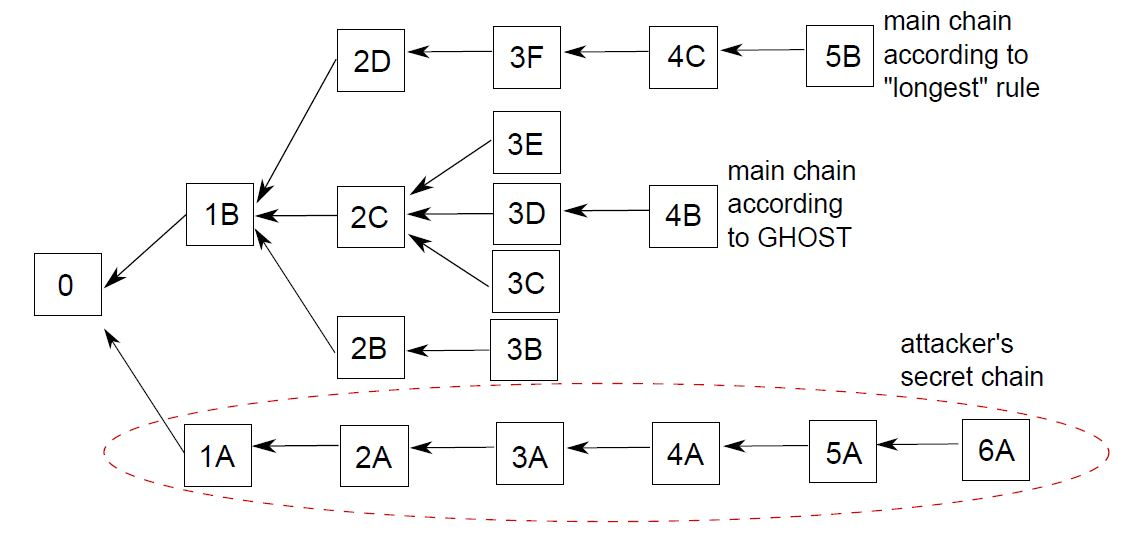
\includegraphics[width=0.8\textwidth,angle=0]{images/forking-risks}
     \caption{Auswahl der gültigen Blockchain. In Bitcoin die längere Blockchain. In Ethereum die Blockchain }
    \label{fig:forking-risks}
\end{figure} 

%Das Problem der Benachteiligung der Miner wird dadurch gelöst, dass es ihnen möglich ist zu entscheiden, ob sie einen neu gefunden Block ignorieren. Mit Bezug zum oberen Beispiel: Miner A, mit 45\% der Rechenleistung, findet einen Block und  alle anderen Nodes erhalten diesen nach 4 Sekunden. Die Wahrscheinlichkeit sehr gering ist, dass sie innerhalb von einer Sekunde einen Block finden welchen sie an den neuen anhängen können. Deshalb entscheiden sich die Nodes dazu den Block zu ignorieren, und arbeiten mit 55\% der Rechenleistung weiter am alten Block. Dies führt dazu, dass sie 

\paragraph{Schlechtere Skalierbarkeit durch Smart Contracts}
%TODO: S.21 Scherer: Sharing Explanation einbauen ?
Ethereum löst die Probleme von häufig auftretenden Forks und erlaubt so einen höheren Transaktionsdurchsatz sowie schnellere Transaktionsbestätigungszeiten. Weitere Probleme entstehen jedoch, wenn eine Blockchain nicht nur Geldtransfertransaktionen verarbeitet. Ethereum erlaubt das speichern und ausführen von eigenem Code durch Smart Contracts. Dadurch steigt die Komplexität der auszuführenden Transaktionen. Dadurch nimmt die Skalierbarkeit ab, da die entstehenden größeren Blöcke eine längere Propagationszeit verursachen. Ebenfalls verschlechtert sich die Performance des Netzwerks, da die Daten schwieriger zu verarbeiten sind. So muss jede Node alle Transaktionen verifizieren, Smart Contract-Code ausführen, und die Ergebnisse speichern. \cite{SchererPerformanceScalabilityBlockchain2017}. 

%TODO: Double Spend Angriff durch erstellen von 2 Transaktionen in Grundlagen erklären
In Ethereum werden Transaktionen sequentiell bei allen Nodes ausgeführt. Dazu gehört das ausführen von Smart Contract-Code sowie das verifizieren der Ergebnisse. Nur so können in Konflikt stehende Transaktionen, wie zum Beispiel beim Double-Spend) erkannt werden. Eine Parallelausführung ist nicht möglich. Dies verschlechtert letztendlich die Performance des Netzwerks, da es länger dauert Transaktionen auszuführen \cite{SchererPerformanceScalabilityBlockchain2017}. Dies wird auch durch ein Beispiel klar. Ein Angreifer kann DoS-Attacken ausführen, indem er komplex auszuführende Smart Contracts schreiben. Die Ausführung von diesem bei jeder Node führt dazu, dass keine anderen Operationen ausgeführt werden können. Ethereum löst dieses Problem, indem der Transaktionssender für jeden Berechnungschritt eine Gebühr zahlen muss. Dies funktioniert jedoch nur, wenn in der Blockchain-Anwendung eine Kryptowährung genutzt wird \cite{VukolicRethinkingPermissionedBlockchains2017}. 

Ebenfalls behauptet Vukolic, dass der Code der Smart Contracts nicht bei allen Nodes ausgeführt werden muss. Um Konsens zu erreichen genügt es, dass alle Nodes den gleichen Stand der Daten erhalten. Deshalb könnte die Codeausführung von nur von bestimmten Nodes ausgeführt werden. Das Problem dabei ist, dass man eine genügend große Anzahl an vertrauenswürdige Teilnehmer festlegen muss \cite{VukolicRethinkingPermissionedBlockchains2017}. Damit geht allerdings auch das vertrauenslose Modell der Blockchain verloren.

%TODO: Lightning Network ?
%TODO: Weiterführende Quellen für Netzwerktopologien ?
%TODO: Bearbeiten, wenn vorheriges Kapitel fertig
Letztendlich lässt sich sagen, dass Public Blockchains nicht skalieren. Um dies zu lösen, müsste die Netzwerktopologie verbessert werden um schnelle Blockpropagrationszeiten zu erlauben \cite{SchererPerformanceScalabilityBlockchain2017}. Weitere Schwierigkeiten bestehen sobald nicht nur Geldtransferaktionen verarbeitet werden müssen. Betrachtet man das CAP-Theorem wird ersichtlich, dass nur die Eigenschaften Dezentralisierbarkeit und Sicherheit gegeben sind. Es ist jedoch zu bedenken, dass viele Probleme der Skalierbarkeit aufgrund der genutzten Konsensmechanik bestehen. Auch wenn es teilweise Lösungsvorschläge für diese gibt, genügen sie bisher nicht um Skalierbarkeit herzustellen. Deshalb gilt es, die Limitationen von Permissioned Blockchains sowie alternative Konsensmechaniken für diese zu analysieren.

%TODO: S.23 Scherer: "The bottom line is that public networks are not efficient"
%TODO: MinPermissioned: Introduces a concept for better throughput, but it is not tested (??)
%TODO: S.1-6 LiScalable: Introducing a concept with sattelite chains

\subsection{Permissioned Blockchains}
%TODO: Governing authority erwähnen ?
Permissioned Blockchains werden eingesetzt, wenn nur bestimmte Teilnehmer an der Blockchain teilnehmen sollen. Dadruch entsteht eine stärkere Zentralisierung als bei Public Blockchains. Bezieht man sich auf das CAP-Theorem, müssten sich dadurch die Sicherheit und/oder Skalierbarkeit verbessern. Dies führt allerdings auch dazu, dass ein größeres Maß an Vertrauen zwischen den Teilnehmern gegeben sein muss. Dies wird dadurch sichergestellt, dass jeder Teilnehmer die Rechte zur Teilnahme am Netzwerk erhalten hat und die Identitäten dieser bekannt. Duch letzteres ist nachverfolgbar, welche Teilnehmer welche Transaktionen ausführt \cite{SchererPerformanceScalabilityBlockchain2017}.

%TODO: Aufgabe von Commiter und Ordering Service genauer betrachten
%TODO: Ist noch Konsens gegeben wenn jede Transaktion von einen anderen Peer ausgeführt wird ? Was wenn das Ergebnis einer Transaktion von einem Peer verfälscht wird ?
 dass das höhere Vertrauen es erlaubt den Nodes verschiedene Aufgaben zuzuteilen. Dies beschreibt er am Beispiel von Hyperledger Fabric, einer Permissioned-Blockchain. In dieser gibt es Peer Nodes, und Ordering Nodes. Erstere übernehmen das ausführen von Code, während letztere die Reihenfolge der auszuführenden Transaktionen in den Blöcken bestimmten und dadurch ebenfalls überprüfen ob es in Konflikt stehende Transaktionen gibt (Genauer im Kapitel \ref{sec:hyperledger-fabric-composer}. Im Gegensatz zu Ethereum können Peer Nodes so parallel Transaktionen verarbeiten. Sie müssen sich nicht um eventuelle Konflikte oder die Reihenfolge der Transaktionen kümmern. Letztendlich würde die Skalierbarkeit, im Rahmen des Verarbeitens von Transaktionen, nur von der Hardware der Peers abhängen \cite{SchererPerformanceScalabilityBlockchain2017}.

%TODO: Paper mit Transaktionswerten
Dies wird ebenfalls im Paper von ... bestätigt

Letztendlich lässt sich sagen, dass sich bei Permissioned Blockchains das CAP-Theorem bezüglich der Skalierbarkeit, im Rahmen des Verarbeitens von Transaktionen, bestätigt. Diese ist jedoch ebenfalls von dem genutzten Konsensmechanismus abhängig. Weiterhin muss das CAP-Theorem noch auf die Sicherheit untersucht werden. Deshalb erfolgt im nächsten Kapitel die Analyse der Skalierbarkeit und Sicherheit von Konsensmechanismen.

%TODO: S.26-28 Scherer: TPS Performance of Fabric
%TODO: S.29-30 Scherer: Scalability Discussion: Throughput with more powerful computers, endorsers, etc.
%TODO: S.31 Scherer: Conclusion is that the question of the fabric performance is not answered
%TODO: S. 1-6 Pongnumkul: Performance ANalysis of Ethereum and Fabric. But how many Participants ? Only private chain ?
%TODO: S.3 Sukhwani: PBFT Performance in Fabric
%TODO: S.2 LiScalable: Blockchain Sharding

\label{subsec:eval-konsens}
\section{Konsensmechanismen}
%TODO: Sacrificing Decentralisiation means we need more trust in the nodes-->This leads to kind of a governing authority-->No problem to implement sharding and channels --> With the given trust, less trust needs to be guaranteed by the consensus mechanism --> We can use other mechanisms (Scherer, S.21)
%TODO: Quelle prüfen (GramoliDanger)
Eine Blockchain, welche den Proof-of-Work als Konsensmechanismus nutzt, ist nicht skalierbar. Ebenfalls würde er in Netzwerken mit relativ wenig Teilnehmern die Sicherheit beeinträchtigen, da ein Teilnehmer einfacher 51\% der Rechenleistung erreichen kann \cite{Gramolidangerprivateblockchains2016}. Für Permissioned Blockchains muss also ein Konsensmechanismus gefunden werden, welche Skalierbarkeit und Sicherheit herstellt. Aufgrund des höheren Vertrauens in diesen behauptet Scherer, dass ein Konsensmechanismus genutzt werden kann, welcher Vertrauen in geringerem Maße als der Proof-of-Work herstellt. Somit könnten Skalierbarkeit und Sicherheit hergestellt werden \cite{SchererPerformanceScalabilityBlockchain2017}. Im folgenden werden die Konsensmechanismen a, b, und c miteinander verglichen und evaluiert.

%TODO: S.1-4 Gramoli: PoW in Permissioned Chains can be dangerous
%TODO: S.8 ZhengBlockchainChallenges: Consensus Algorithm Byzantine Generals Erklärung
%TODO: S.10-11 ZhengBlockchainChallenges: Consensus Comparison
%TODO: S.4 ZhengBlockchainChallenges: Proof of Stake --> Rich get richer
%TODO: S.7 WustYouNeed: PBFT Consensus is enough for permissioned blockchains
%TODO: S.117 CromanScaling: PBFT could be enough for permissioned blockchains
%TODO: S.22 Scherer: Bitcoin PoW Problems
%TODO: S.3 BenHamida Consensus Algorithms Proof of Elapsed Time, Voting Consensus, PBFT, FBA, Terndermint, Diversity Mining
%TODO: S.6 BenHamida Consensus Zusammenschluss von Minern/Votern etc.
%TODO: S.3-4 Cachin: Theorie eines Konsensmechanismus
%TODO: S.10-24 Cachin: Consens Algorithms
%TODO: S.1-11 PBFT vs PoA: PBFT is better, because...
%TODO: S.2 SankarSurvery: Stellar Consensuns and PBFT of Hyperledger
%TODO: S.1-14 VukolicQuest: Proof of Work vs BFT
%TODO: Check R3 Consens Algorithm

\section{Sonstige}

\subsection{Private Transaktionen}
%TODO: S.2 WustYouNeedBlockchain: Tensio between Transparency and Privacy
%TODO: Private Channels in Fabric
%TODO: Private Transactions in Quorum

\subsection{Code Execution}
%S.2 VukolicRethinking: Non-Deterministic Execution

\subsection{Datenmenge}

%TODO: Scherer: "With increased block size comes a larger blockchain, which means the blockchain could get too large in size that not everyone can run a full node. This means that 23(41) only large scale server can run a full node, leaving the average user behind, and therefore resulting in less decentralization."
%TODO: S.6 BenHamida Real-time analysis and reaction on data (?)
%TODO: Sensorwerte usw. Vertrauen (?)
%TODO: Redundanz der Daten --> Weniger Full Nodes --> Weniger Dezentralisierung --> Höhere Wahrscheinlichkeit eines Zusammenschlusses um Rechenpower zu erreichen
%TODO: Datenmenge und Redundanz





